\chapter{Bevezetés}
Ebben a dolgozatban a BME VIK Villamosmérnök MSc képzés Önálló Laboratórium 1 c. tárgyának keretében végzett kutatási és tervezési munkámat összegzem. A dolgozatom témája egy kevéssé ismert nyomtatott antennatípus, a BIFA (Balanced Inverted F Antenna) tervezése.
\section{BIFA}
\par A BIFA antennatípus nem gyakori a szakirodalomban, az irodalomkutatás során csak a Silicon Laboratories egy 2014-es application note-jában \cite{an847} találkoztam vele. Ez az antennatípus egy variációja az IFA-nak (Inverted F Antenna), ezért az IFA jellegzetességeiből kiindulva érdemes tárgyalni.
\begin{figure}[h]
	\centering
	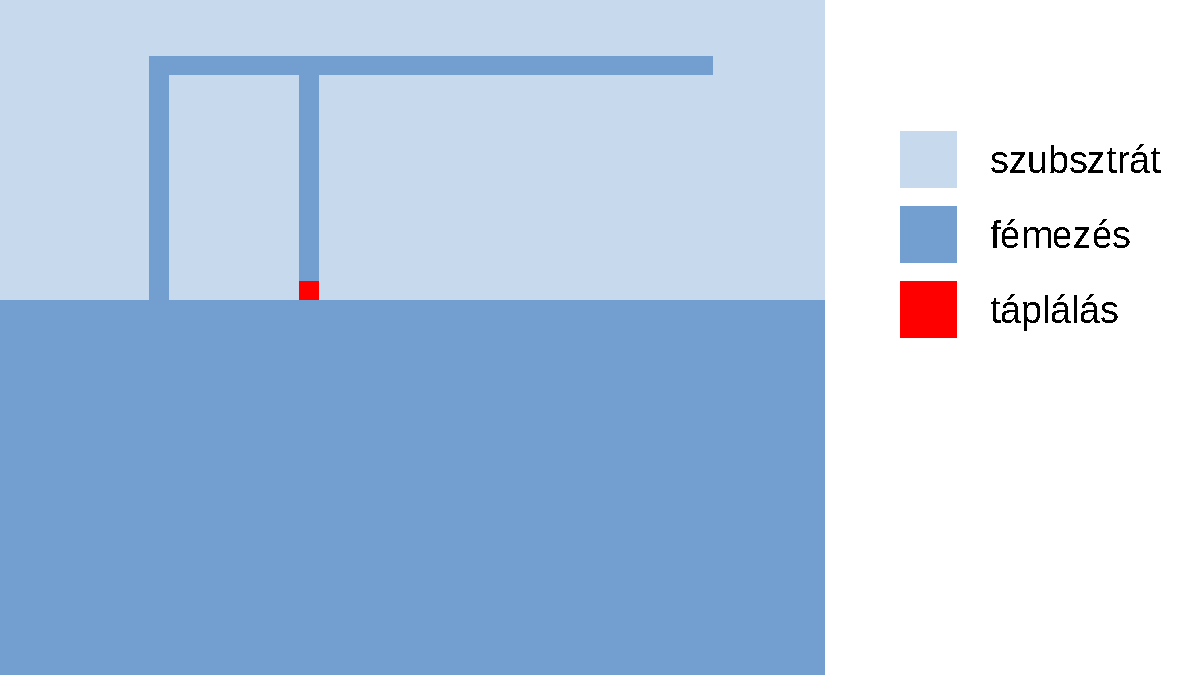
\includegraphics[width=0.6\textwidth]{kep/tipikus_ifa.pdf}
	\caption{Egy tipikus IFA egy nyomtatott áramköri lap szélén.}
	\label{fig:tipikus_ifa}
\end{figure}
\par Az IFA az ILA (Inverted L Antenna)  egy variációja (\ref{fig:tipikus_ila}. ábra). Az IFA előnye az ILA-val szemben a megnövekedett abszolút értékű bemeneti impedancia, ami miatt a működési hullámhosszhoz képest kis méretben is jobban használható, könnyebben illeszthető a tápláló hálózathoz. Ezek miatt az IFA-t szélesebb körben alkalmazzák, például mobil eszközökben, ahol az antenna számára rendelkezésre álló hely erősen korlátozott \cite{multi-band}, ekkor bizonyos esetekben a nyomtatott áramköri lapon (NYÁK) kialakított, megfelelő alakú fémezés maga az antenna.
\begin{figure}[h]
	\centering
	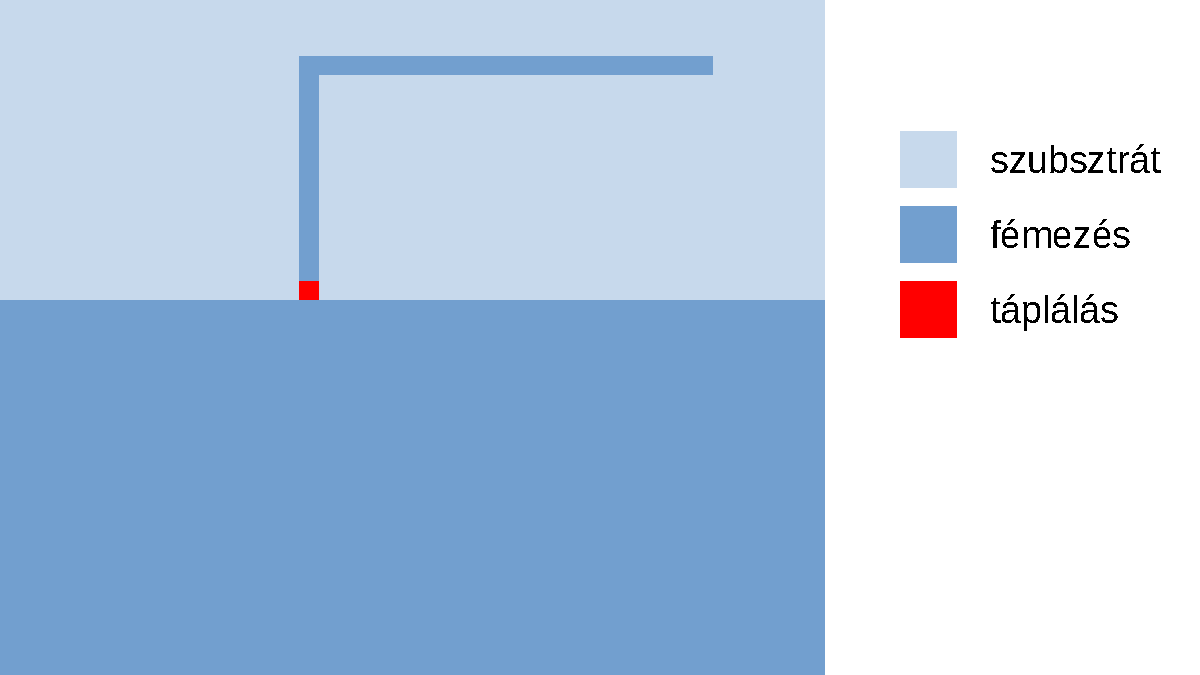
\includegraphics[width=0.6\textwidth]{kep/tipikus_ila.pdf}
	\caption{Egy tipikus ILA egy nyomtatott áramköri lap szélén.}
	\label{fig:tipikus_ila}
\end{figure}
\par Az IFA alapvetően egy monopól típusú antenna, emiatt aszimmetrikus táplálású (\ref{fig:tipikus_ifa}. ábra). A monopól (monopólus) antennákat általában olyankor alkalmazzák, amikor az antenna környezetében egy az antennához képest nagy kiterjedésű vezető található, az ún. alaplap, amit ki lehet használni az antenna sugárzási tulajdonságainak javítására. Ideális esetben az alaplap egy végtelen kiterjedésű végtelen vezetőképességű sík. Ekkor a helyettesítő töltések módszerével \cite{fodor} az alaplapot eltávolítva és a monopól az alaplap síkjára tükrözött képét behelyettesítve egy (a középpontjában a monopóléhoz képest kétszeres feszültséggel gerjesztett) dipól (dipólus) antennát kapunk, amelynek egyik szára az eredeti monopól, ahogy az \aref{fig:monopol}. ábrán látható.
\begin{figure}[h]
	\centering
	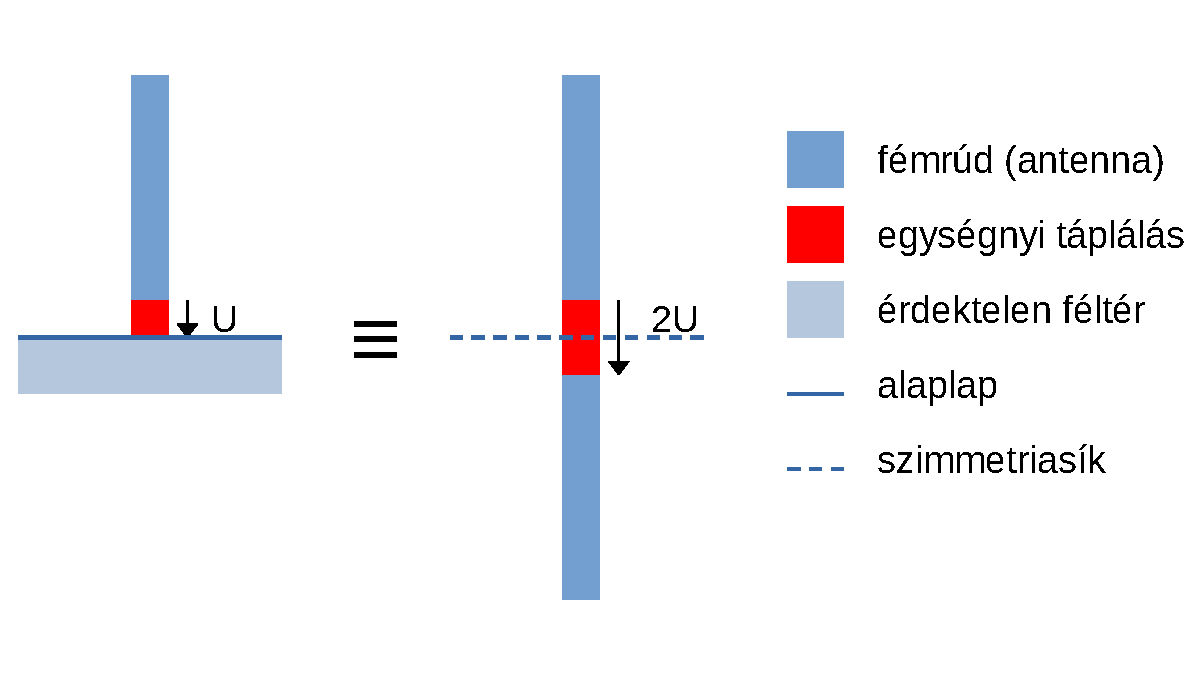
\includegraphics[width=0.6\textwidth]{kep/monopol.pdf}
	\caption{Ideális monopól és ekvivalens dipól.}
	\label{fig:monopol}
\end{figure}
\par Az így kapott antenna az alaplap síkja fölött a monopóluséval megegyező sugárzási karakterisztikát produkál. A monopól esetén az ekvivalens dipól másik szárát az alaplapban indukált áramok hatása helyettesíti, így jön létre a megegyező sugárzási karakterisztika.
\par A fenti helyettesítési módszer nem mindig használható, például egy NYÁK-on kialakított nyomtatott antenna esetén nem, hiszen ekkor legfeljebb a NYÁK földkitöltése tekinthető nagy kiterjedésű vezetőnek, de ez messze nem végtelen kiterjedésű, ráadásul az antenna a földkitöltés síkjában helyezkedik el.
\section{Céges háttér}

